\section{Rejoindre le réseau}

L'algorithme pour rejoindre le réseau est, dans \SPRAY, la seule manière
d'introduire de nouveaux arcs dans le réseau. Afin de répondre à la première
partie de l'énoncé du problème (\REF), ce nombre d'arcs doit augmenter
logarithmiquement comparé à la taille du réseau. Tout comme dans \SCAMP, nous
supposons que chacuns des pairs respecte cette contrainte. Dès lors, ces
derniers utilisent ce savoir afin de propager l'identité du nouvel
arrivant. L'algorithme~\ref{algo:joining} décrit la façon dont le contact envoie
la nouvelle identité à son voisinage où elle est intégrée directement à leur vue
partielle. En définitive, le nombre d'arcs dans le réseau augmente de
$1+\ln(|\mathcal{N}|)$ et ce, seulement en utilisant des interactions de voisin
à voisin.

\begin{figure*}
  \centering
  \subfloat[Figure A][$p_1$ contacts $p_2$ to join the network. $p_1$ adds
  $p_2$ to its neighborhood. $p_1$ sends its request to $p_2$.]{
    
\begin{tikzpicture}[scale=1.2]

  \newcommand\X{35pt};
  \newcommand\Y{15pt};

  \draw(-0.75*\X, 0pt); %% positioning
  \draw( 2.75*\X, 0pt); %% positioning

  \scriptsize
  \draw[->,dashed,very thick, color=darkblue](5+0*\X, 0*\Y) -- 
  node[anchor=south]{(a)}(-5+ 2*\X, 0*\Y);
  \draw[->] (-5+2*\X, 5pt) -- (5+\X, \Y);
  \draw[->] (-5+2*\X, 5pt) --  (5+\X, 2*\Y);
  \draw[->] (-5+2*\X, -5pt) -- (5+\X, -\Y);
  \draw[->] (-5+2*\X, -5pt) -- (5+\X, -2*\Y);

  \normalsize
  \draw[fill=white, very thick, draw=darkblue]
  (0*\X, 0*\Y) node{\DARKBLUE{$n_1$}} +(-5pt,-5pt) rectangle +(5pt,5pt);
  \draw[fill=white, very thick]
  (2*\X, 0*\Y) node{$n_2$} +(-5pt,-5pt) rectangle +(5pt,5pt);

  \draw[fill=white](1*\X,2*\Y) node{$n_6$} +(-5pt,-5pt) rectangle +(5pt,5pt);
  \draw[fill=white](1*\X,1*\Y) node{$n_5$} +(-5pt,-5pt) rectangle +(5pt,5pt);
  \draw[fill=white](1*\X,-1*\Y) node{$n_4$} +(-5pt,-5pt) rectangle +(5pt,5pt);
  \draw[fill=white](1*\X,-2*\Y) node{$n_3$} +(-5pt,-5pt) rectangle +(5pt,5pt);
  
\end{tikzpicture}}
  \hspace{8pt}
  \subfloat[Figure B][The $onSubs(p_1)$ event is raised at $p_1$
  which forwards the subscription to $p_1$'s neighborhood.]{
    
\begin{tikzpicture}[scale=1.2]

  \newcommand\X{35pt};
  \newcommand\Y{15pt};

  \draw(-0.75*\X, 0pt); %% positioning
  \draw( 2.75*\X, 0pt); %% positioning

  \scriptsize
  \draw[->](5+0*\X, 0*\Y) -- (-5+ 2*\X, 0*\Y);
  \draw[->, very thick, color=darkblue] (-5+2*\X, 5pt) -- (5+\X, \Y);
  \draw[->, very thick, color=darkblue] (-5+2*\X, 5pt) --
  node[anchor=south west]{(b)} (5+\X, 2*\Y);
  \draw[->, very thick, color=darkblue] (-5+2*\X, -5pt) -- (5+\X, -\Y);
  \draw[->, very thick, color=darkblue] (-5+2*\X, -5pt) --
  node[anchor=north west]{(b)}(5+\X, -2*\Y);

  \normalsize
  \draw[fill=white]
  (0*\X, 0*\Y) node{$n_1$} +(-5pt,-5pt) rectangle +(5pt,5pt);
  \draw[fill=white, very thick, draw=darkblue]
  (2*\X, 0*\Y) node{\DARKBLUE{$n_2$}} +(-5pt,-5pt) rectangle +(5pt,5pt);

  \draw[fill=white, very thick]
  (1*\X,2*\Y) node{$n_6$} +(-5pt,-5pt) rectangle +(5pt,5pt);
  \draw[fill=white, very thick]
  (1*\X,1*\Y) node{$n_5$} +(-5pt,-5pt) rectangle +(5pt,5pt);
  \draw[fill=white, very thick]
  (1*\X,-1*\Y) node{$n_4$} +(-5pt,-5pt) rectangle +(5pt,5pt);
  \draw[fill=white, very thick]
  (1*\X,-2*\Y) node{$n_3$} +(-5pt,-5pt) rectangle +(5pt,5pt);

\end{tikzpicture}}
  \hspace{8pt}
  \subfloat[Figure C][The $onFwdSubs(p_1)$ event is raised at $p_{3-6}$. The
  peers add $p_1$ to their neighborhood.]{
    
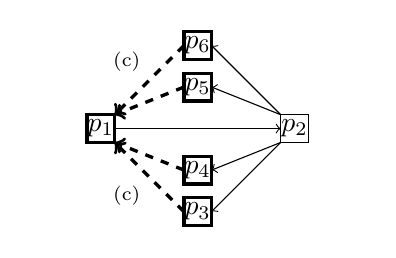
\begin{tikzpicture}[scale=1]

  \newcommand\X{35pt};
  \newcommand\Y{15pt};

  \draw(-0.75*\X, 0pt); %% positioning
  \draw( 2.75*\X, 0pt); %% positioning

  \scriptsize
  \draw[->](5+0*\X, 0*\Y) -- (-5+ 2*\X, 0*\Y);
  \draw[->] (-5+2*\X, 5pt) -- (5+\X, \Y);
  \draw[->] (-5+2*\X, 5pt) -- (5+\X, 2*\Y);
  \draw[->] (-5+2*\X, -5pt) -- (5+\X, -\Y);
  \draw[->] (-5+2*\X, -5pt) -- (5+\X, -2*\Y);

  \draw[->,dashed, very thick](-5+\X, 2*\Y) --
  node[anchor=south east]{(c)} ( 5pt,5pt);
  \draw[->,dashed, very thick](-5+\X, 1*\Y) -- ( 5pt,5pt);
  \draw[->,dashed, very thick](-5+\X, -1*\Y) -- ( 5pt,-5pt);
  \draw[->,dashed, very thick](-5+\X, -2*\Y) --
  node[anchor=north east]{(c)}( 5pt,-5pt);

  \normalsize
  \draw[fill=white, very thick]
  (0*\X, 0*\Y) node{$p_1$} +(-5pt,-5pt) rectangle +(5pt,5pt);
  \draw[fill=white]
  (2*\X, 0*\Y) node{$p_2$} +(-5pt,-5pt) rectangle +(5pt,5pt);

  \draw[fill=white, very thick]
  (1*\X,2*\Y) node{$p_6$} +(-5pt,-5pt) rectangle +(5pt,5pt);
  \draw[fill=white, very thick]
  (1*\X,1*\Y) node{$p_5$} +(-5pt,-5pt) rectangle +(5pt,5pt);
  \draw[fill=white, very thick]
  (1*\X,-1*\Y) node{$p_4$} +(-5pt,-5pt) rectangle +(5pt,5pt);
  \draw[fill=white, very thick]
  (1*\X,-2*\Y) node{$p_3$} +(-5pt,-5pt) rectangle +(5pt,5pt);
 

\end{tikzpicture}}
  \caption{\label{net:fig:joiningexample}Example of the \SPRAY's joining
    protocol.}
\end{figure*}

\begin{algorithm}

\small
\algrenewcommand{\algorithmiccomment}[1]{\hskip2em$\rhd$ #1}

\newcommand{\comment}[1]{$\rhd$ #1}


\algblockdefx[initially]{initially}{endInitially}
  [0] {\textbf{INITIALLY:}} 

\algblockdefx[pas]{pas}{endPas}
  [0] {\textbf{EVENTS:}}

\newcommand{\LINEFOR}[2]{%
  \algorithmicfor\ {#1}\ \algorithmicdo\ {#2} %
  }

\newcommand{\LINEIFTHEN}[2]{%
  \algorithmicif\ {#1}\ \algorithmicthen\ {#2} %
  }

\newcommand{\INDSTATE}[1][1]{\State\hspace{\algorithmicindent}}

\begin{algorithmic}[1]
  \Statex
  \initially
    \State $\mathcal{P} \leftarrow \varnothing$;
    \hfill \comment{the partial view is a multiset}
    \State $p$ ; \hfill \comment{identity of the local peer}
  \endInitially
  
  \pas
  \Function{onSubs}{$o$} \hfill \comment{$o: origin$}
    \State \LINEFOR{\textbf{each} $\langle q,\,\_\, \rangle \in\mathcal{P}$}
    {$sendTo(q,\, 'fwdSubs',\, o)$;} \label{line:multicast}
    \EndFunction
    \Statex
    \Function{onFwdSubs}{$o$} \hfill \comment{$o: origin$}
    \State $\mathcal{P} \leftarrow
    \mathcal{P}\uplus \left\{\langle o,\, 0 \rangle\right\}$;
    \EndFunction
  \endPas
  
\end{algorithmic}

\caption{\label{net:algo:joining}The joining protocol of \SPRAY.}
\end{algorithm}

La vue partielle est un multiensemble de couples $\langle n,\, age\rangle$ qui
associe à chaque voisin $n$ l'âge $age$. Ce multiensemble permet de gérer les
doublons. L'âge joue le même rôle que dans \CYCLON, çàd qu'il accélère la
suppression des pairs qui sont sortis ou ont crash. L'évenement $onSubs$ est
appelé chaque fois qu'un pair rejoins le réseau via ce contact. $onSubs$
redirige l'identité du pairs à tous ses voisins, indépendament de
l'âge. L'évenement $onFwdSubs$ est déclanché lorsqu'un pair reçoit une telle
identité redirigée. $onFwdSubs$ ajoute la référence en initialisant son âge à
$0$.

La figure~\ref{net:fig:joiningexample} décrit un scenario où le pair $p_1$ contacte
le pair $p_2$ afin de rejoindre le réseau composé de $\{p_2$, $p_2$, $p_4$,
$p_5$, $p_6\}$. Pour simplifier, la figure ne montre que les arcs nouvellement
introduit ainsi que le voisinage de $p_1$ et $p_2$. Le pair $p_1$ ajoute
directement $p_2$ dans sa vue partielle. Ce dernier redirige l'identité de $p_1$
à chacun de ses voisins.  Chacun de ces voisins ajoute alors $p_1$ à leur vue
partielle. Au total, \SPRAY établie 5 connexions. Le réseau en résultant est
connecté.

Malheureusement, les vues partiels des derniers arrivant sont clairement
déséquilibrés comparé au reste du réseau. De ce fait, ils violent la première
condition de l'énoncé du problème (\REF). Le processus de mélange décrit dans la
prochaine section a pour but de ré-équilibrer les vues partielles.


%%% Local Variables:
%%% mode: latex
%%% TeX-master: "../../paper"
%%% End:
